\documentclass[conference]{IEEEtran}
\IEEEoverridecommandlockouts
\usepackage{cite}
\usepackage{amsmath,amssymb,amsfonts}
\usepackage{algorithmic}
\usepackage{graphicx}
\usepackage{textcomp}
\usepackage{xcolor}
\def\BibTeX{{\rm B\kern-.05em{\sc i\kern-.025em b}\kern-.08em
		T\kern-.1667em\lower.7ex\hbox{E}\kern-.125emX}}
\begin{document}
	
	\title{Integration of 75MW Solar PV Plant: Transmission System Design Analysis}
	
	\author{\IEEEauthorblockN{Brent Dickinson}
		\IEEEauthorblockN{Tianci Xi}
	}
	
	\maketitle
	
\begin{abstract}
	This report presents the design and analysis of transmission system modifications required to integrate a new 75MW solar PV plant while addressing existing system reliability concerns. The study evaluates various transmission line and transformer options to determine the most cost-effective solution that maintains system stability under both normal and N-1 contingency conditions.
\end{abstract}

\section{Introduction}
The integration of renewable energy sources into existing power grids presents technical challenges. We analyze the design requirements and potential solutions for integrating a new 75 MW utility-scale solar photo-voltaic (PV) facility into an existing 37-bus power system while also solving current reliability issues.

We aim to find the most cost-effective transmission system additions required to integrate 75 MW of solar generation at the NEWSOLAR substation. That goal is subordinate to the constraints of ensuring system reliability through dual transmission paths to the facility and resolving existing system violations identified using PowerWorld's contingency analysis.

The design must satisfy the following constraints. Bus voltages must be maintained between 0.95 and 1.10 per unit, while keeping all line flows below 100\% of their thermal limits. The system must maintain stability under both normal operation and N-1 contingency conditions. Additionally, redundant transmission paths to the NEWSOLAR substation are required. The system must accommodate the solar plant operating at both full capacity (75 MW) and offline conditions.

Our approach incorporates contingency analysis, evaluation of available transmission corridors and voltage levels, and assessment of various conductor types and their associated costs. We consider transformer options and substation modifications. We conduct an economic analysis incorporating both capital costs and five-year loss reduction benefits.

Initial contingency analysis reveals specific reliability concerns in the OAK69-BUCKEYE69-APPLE69 corridor, which must be addressed alongside the integration of the new solar facility. The following sections detail the technical analysis, proposed solutions, and economic justification for the recommended design.

\section{Initial System Analysis}
\subsection{Base Case Evaluation}
The existing 37-bus system operates with a total load of 826.3 MW and 275.5 Mvar, served by ten generators producing 837.7 MW. System losses are approximately 10.7 MW, representing 1.3\% of total generation, which indicates reasonably efficient power delivery under normal conditions. The system maintains adequate reactive power compensation through nine switched shunts, collectively providing -122.5 Mvar of reactive support.

PowerWorld's case summary for the existing system is shown in Figure \ref{fig:casesummaryexisting}
\begin{figure}[tbph]
	\centering
	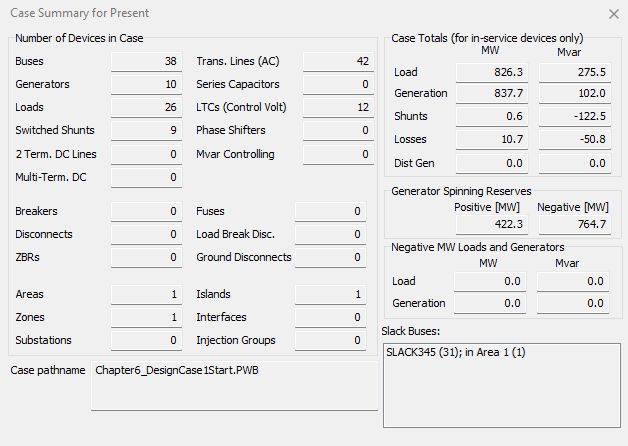
\includegraphics[width=1\linewidth]{figures/case_summary_existing}
	\caption{Case summary for existing system}
	\label{fig:casesummaryexisting}
\end{figure}
\subsection{Contingency Analysis}
PowerWorld's contingency analysis examines conditions when each element of the power system is taken offline. It reveals vulnerability in the 69 kV network in three contingency violations. Specifically, loss of either the PINE138 transformer or the PINE69-APPLE69 line results in overload, with the OAK69-BUCKEYE69 line experiencing loading up to 110.8\% of its thermal limit. These violations suggest that the existing infrastructure is approaching its capacity limits. 

These results are summarized in Table \ref{tab:violations}. A zoomed-in view of the affected areas of the power system is shown in Figure \ref{fig:baseviolations}.
\begin{table}[htbp]
	\caption{Line violations in contingency analysis}
	\begin{center}
		\begin{tabular}{|l|c|c|c|}
			\hline
			\textbf{Contingency} & \textbf{Flow(A)} & \textbf{Limit(A)} & \textbf{\%} \\
			\hline
			\textit{PINE138-PINE69 Xfmr:} & & & \\
			OAK69-BUCKEYE69 & 760.3 & 686.1 & 110.8 \\
			BUCKEYE69-APPLE69 & 454.2 & 418.4 & 108.6 \\
			\hline
			\textit{PINE69-APPLE69 Line:} & & & \\
			OAK69-BUCKEYE69 & 699.2 & 686.1 & 101.9 \\
			\hline
		\end{tabular}
		\label{tab:violations}
	\end{center}
\end{table}
\begin{figure}[tbph]
	\centering
	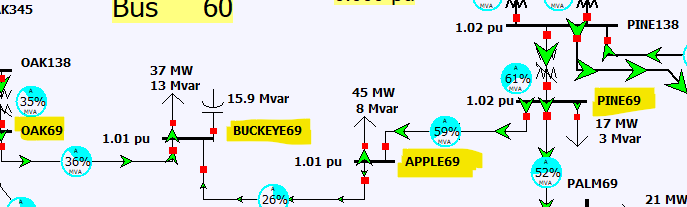
\includegraphics[width=1\linewidth]{figures/base_violations}
	\caption{Existing contingency violations - problem area}
	\label{fig:baseviolations}
\end{figure}
\section{Design}
The design solution must incorporate new transmission infrastructure to connect the 75 MW solar facility at NEWSOLAR while simultaneously addressing existing problems. There must be redundant transmission paths to NEWSOLAR for reliability, meaning at least two separate transmission lines must be constructed. These lines can be either 69 kV or 138 kV, with NEWSOLAR and all existing substations capable of accommodating either voltage level through installation of transformers. The system must maintain all bus voltages between 0.95 and 1.10 per unit and keep all line flows below their thermal limits under both normal operation and any single-contingency (N-1) scenario.

The optimal solution will minimize total cost, calculated as the construction costs minus any savings from reduced system losses over a 5-year period at \$60/MWh. Construction costs include both fixed components (\$1.25M for 138 kV or \$750k for 69 kV lines) and variable costs based on distance and conductor type. If 138 kV is utilized, additional costs include substation upgrades (\$900k per substation) and necessary transformers (\$1.5M for 101 MVA or \$1.8M for 168 MVA). The solution must resolve existing contingency violations, particularly the overloads observed in the OAK69-BUCKEYE69-APPLE69 corridor, while ensuring reliable operation both when the solar plant is at full output and when it is offline.
\subsection{Transmission Line Parameters}
A note on how to input transmission line parameters into PowerWorld is in order. Table A.4 in the text gives resistance in ohms per conductor per mile for 50$^\circ$C at 60Hz as well as series inductance (ohms/mile/conductor for 1 foot spacing) and shunt capacitance (S/mile/conductor for 1 foot spacing). Resistance pulled from Table A.4 can be used directly in the "Calculate Impedances" dialog box in PowerWorld. But for 69kV lines, the three phases are spaced 2m apart and 4m apart for 138kV lines. We need a way to convert the 1-foot spacing parameters appropriately. Assuming equilateral spacing of lines, Equation 4.5.9 \cite{glover2007} in the text suggests a simple way to adjust series per-mile impedance from the table:
\begin{flalign}
	X_{2m} &= X_{1ft}\cdot\frac{\ln\left(\frac{2\times3.28}{\text{GMR}}\right)}{\ln\left(\frac{1}{\text{GMR}}\right)}
\end{flalign}
where GMR comes from the same table for the conductor of interest. 

We calculate shunt susceptance similarly given the 1-foot spacing shunt reactance and outer diameter given in the table:
\begin{flalign}
	B_{2m} & = \frac{\ln(1/r)}{Xc_{1ft}\cdot\ln(2\times3.28/r)}
\end{flalign}
where $r$ is the conductor's outer radius. Though these are stranded conductors, we treat them as solid since the associated error is small. Note that we multiply this value by 3 for 3 phases. 

Table \ref{tab:tl_params} shows parameters for the 69kV lines which go into PowerWorld's Impedance Calculator. We do not include the 138kV lines for reasons explained in the next section.
\begin{table}
	\centering
	\begin{tabular}{|l|c|c|c|}
		\hline
		Parameter & Rook & Crow & Condor \\
		\hline
		R ($\Omega$/mile) & 0.1688 & 0.1482 & 0.1378 \\
		X ($\Omega$/mile) & 0.6421 & 0.6352 & 0.6326 \\
		B (S/mile) & $6.63\times10^{-6}$ & $6.71\times10^{-6}$ & $6.78\times10^{-6}$ \\
		\hline
	\end{tabular}
	\vspace{0.5em}
	\caption{Transmission Line Parameters at 60 Hz, 2m Spacing}
	\label{tab:tl_params}
\end{table}
\subsection{Candidate Solutions}
Table \ref{tab:all_conn} shows all possible NEWSOLAR connections to the network, given the provided set of right-of-way paths available to us. We include cost of installing the least expensive conductors (Rook for 69kV, Crow for 138kV) in the last column. Note that for any 138kV connections, we need to install a 138kV bus with 69-138 transformer at NEWSOLAR. This cost is included in Table \ref{tab:all_conn} and suggests we can eliminate any solution involving those lines; we will connect NEWSOLAR exclusively with 69kV lines unless we are unable to meet the requirements. 

The approach here is to start with the solution involving least total line distance (case 1). We move to solutions involving longer connections only if we run into contingency violations. Further, we use the least expensive conductors to start and upgrade only if needed. 
\begin{table}[h]
	\centering
	\begin{tabular}{|c|l|c|r|}
		\hline
		\textbf{Case} & \textbf{Destination} & \textbf{Total} & \textbf{Total Cost} \\
		\textbf{number} & \textbf{buses} & \textbf{distance (km)} & \textbf{(M\$)} \\
		\hline
		1 & BK69, AP69 & 12 & 5.94 \\
		2 & BK69, OAK69 & 19 & 8.53 \\
		3 & BK69, OAK138 & 19 & 14.37 \\
		4 & AP69, OAK69 & 19 & 8.53 \\
		5 & AP69, OAK138 & 19 & 14.37 \\
		6 & BK69, PIINE69 & 20 & 8.90 \\
		7 & BK69, PINE138 & 20 & 14.90 \\
		8 & AP69, PINE69 & 20 & 8.90 \\
		9 & AP69, PINE138 & 20 & 14.90 \\
		10 & BK69, MP69 & 21 & 9.27 \\
		11 & AP69, MP69 & 21 & 9.27 \\
		12 & OAK69, PINE69 & 27 & 11.49 \\
		13 & OAK69, PINE138 & 27 & 18.36 \\
		14 & OAK138, PINE69 & 27 & 18.36 \\
		15 & OAK138, PINE138 & 27 & 18.36 \\
		16 & OAK69, MP69 & 28 & 11.86 \\
		17 & OAK138, MP69 & 28 & 18.89 \\
		18 & PINE69, MP69 & 29 & 12.23 \\
		19 & PINE138, MP69 & 29 & 19.42 \\
		\hline
	\end{tabular}
	\vspace{0.5em}
	\caption{Possible NEWSOLAR Connections with Line Costs (M\$)}
	\label{tab:all_conn}
\end{table}

We found that simply installing connections to BUCKEYE and APPLE results in several contingency violations. These violations came from over-currents on the OAK-BUCKEYE line we so we replaced that line with Crow conductors to ensure ample allowance for current. With the replaced line we saw no violations. We also saw no violations when we turned off the NEWSOLAR plant in this configuration. 

We see significant power loss savings with this configuration. The screenshot in Figure \ref{fig:case1loss} demonstrates new losses of 9.8MW, a savings of 0.9MW from the base case. To calculate the economic value of this improvement over the five-year period:
\begin{flalign}
	\text{Annual hours} &= 365 \text{ days} \times 24 \text{ hours} = 8760 \text{ hours} \\
	\text{Energy saved} &= 0.9 \text{ MW} \times 8760 \text{ hours/year} \times 5 \text{ years}\nonumber \\
	&= 39,420 \text{ MWh} \\
	\text{Cost savings} &= 39,420 \text{ MWh} \times \$60\text{/MWh}\nonumber \\
	&= \$2.37\text{M}
\end{flalign}
The total cost for case 1 with this upgrade (and including the power loss savings) is shown in Table \ref{tab:cost_breakdown_case1}.
\begin{figure}[h]
	\centering
	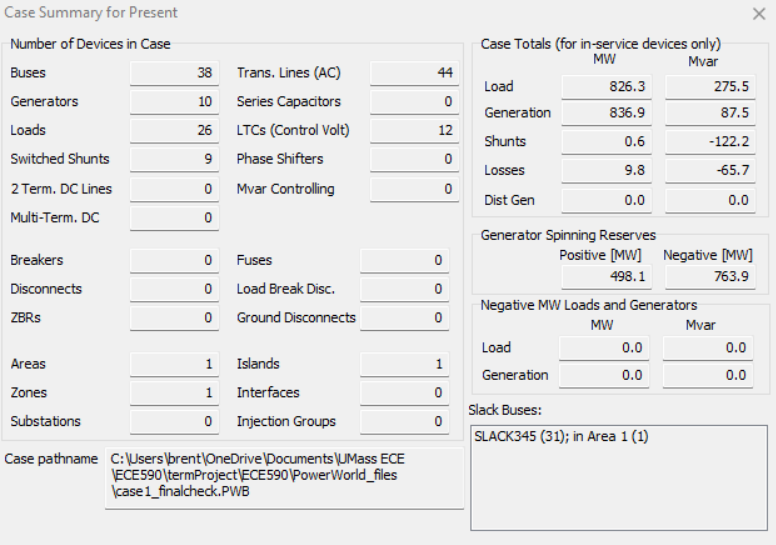
\includegraphics[width=1\linewidth]{figures/case1loss}
	\caption{Case summary for case 1 + upgrade}
	\label{fig:case1loss}
\end{figure}

\begin{table}[h!]
	\centering
	\begin{tabular}{|l|r|}
		\hline
		\textbf{Modification} & \textbf{Cost (M\$)} \\ \hline
		\multicolumn{2}{|l|}{\textbf{Replace OAK-BUCKEYE (69kV Crow)}} \\ 
		\hspace{1em} Fixed Cost & 0.75 \\ 
		\hspace{1em} Variable Cost (\$390,000/km for 8 km) & 3.12 \\ 
		\hspace{1em} \textbf{Total} & \textbf{3.87} \\ \hline
		\multicolumn{2}{|l|}{\textbf{New Line NEWSOLAR-BUCKEYE (69kV Rook)}} \\ 
		\hspace{1em} Fixed Cost & 0.75 \\ 
		\hspace{1em} Variable Cost (\$370,000/km for 6 km) & 2.22 \\ 
		\hspace{1em} \textbf{Total} & \textbf{2.97} \\ \hline
		\multicolumn{2}{|l|}{\textbf{New Line NEWSOLAR-APPLE (69kV Rook)}} \\ 
		\hspace{1em} Fixed Cost & 0.75 \\ 
		\hspace{1em} Variable Cost (\$370,000/km for 6 km) & 2.22 \\ 
		\hspace{1em} \textbf{Total} & \textbf{2.97} \\ \hline
		\textbf{Loss Savings (0.9 MW over 5 years)} & \textbf{-2.37} \\ \hline
		\textbf{Grand Total} & \textbf{7.44} \\ \hline
	\end{tabular}
	\vspace{0.5em}
	\caption{Cost Breakdown for Case 1 Implementation with OAK-BUCKEYE Upgrade}
	\label{tab:cost_breakdown_case1}
\end{table}
We consider cases 2, 4, 6, 8, 10 and 11 as seen in Table \ref{tab:all_conn} because their base cost is in the same neighborhood. Since it is difficult to predict power loss savings, due diligence requires at least a cursory examination. However, the cheapest 6km installation costs \$3M, so for any of these other cases to be preferred there must be no contingency violations. Any corrective line replacement will almost certainly make that option more expensive than case 1 with upgrade. Our approach to this analysis was to install all considered lines and alternately turn on or off the relevant lines, shown in Figure \ref{fig:multi}.
\begin{figure}[h]
	\centering
	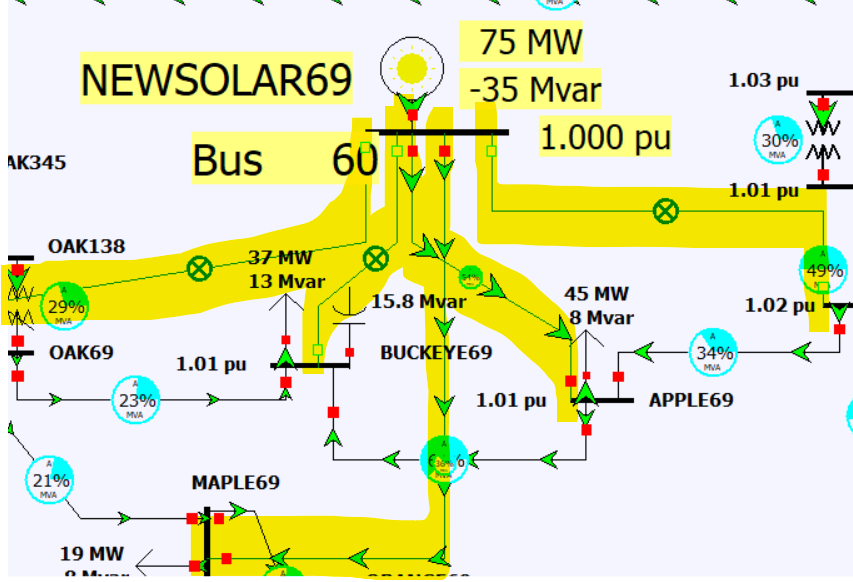
\includegraphics[width=1\linewidth]{figures/multi}
	\caption{Approach to multiple connection analysis}
	\label{fig:multi}
\end{figure}


Case 2 shows four contingency violations related to undervoltage at the OAK 138 \& 345 buses and overcurrent on the BUCKEYE-APPLE line. Case 4 shows the same undervolatge violations as case 2. Case 6 results in the same overcurrent violation observed in the base case (though only when NEWSOLAR is turned off). Cases 8, 10 and 11 all cause overcurrent contingency violations. To correct any of these issues, we would need to install a minimum of 6km of Rook conductors. That makes all these cases more expensive than case 1 plus upgrade.
\section{Conclusion}
Through systematic analysis of 19 possible configurations for the new 75 MW solar facility, we determined that the most cost-effective solution is to connect NEWSOLAR to both BUCKEYE69 and APPLE69 substations using 69 kV lines with Rook conductors, while upgrading the existing OAK69-BUCKEYE69 line using Crow conductors. This configuration, costing \$7.44M, represents the optimal balance between reliability requirements and economic constraints.

The decision to use exclusively 69 kV connections was driven by the substantial cost premium associated with 138 kV options, which required additional substation infrastructure and more expensive conductors. While several other 69 kV configurations appeared comparable in cost, all required remedial upgrades to address contingency violations that ultimately made them more costly than our chosen solution. The upgrade of the OAK69-BUCKEYE69 line to Crow conductors provides sufficient capacity to handle contingency scenarios both with NEWSOLAR at full output and offline, while maintaining all bus voltages and line flows within acceptable limits.

This design successfully achieves all project objectives: it provides redundant transmission paths to the solar facility, resolves existing system violations, maintains system stability under N-1 contingency conditions, and does so at minimum cost. The solution's simplicity and use of standard components should also facilitate maintenance and reduce implementation complexity.
\begin{thebibliography}{9}
	\bibitem{glover2007} J. D. Glover, M. S. Sarma, and T. J. Overbye, \textit{Power Systems Analysis and Design}, 4th ed. Stamford, CT: Cengage Learning, 2007.
\end{thebibliography}
\end{document}